\documentclass[aspectratio=169, 10pt]{beamer}

\usetheme{metropolis}
\metroset{block=fill, numbering=fraction, progressbar=frametitle}

\usepackage[utf8]{inputenc}
\usepackage[T1]{fontenc}
\usepackage[spanish]{babel}
\usepackage{graphicx}
\usepackage{amsmath, amssymb}
\usepackage{xcolor}

\graphicspath{{../ej1/results/pca/}}

\definecolor{accent}{HTML}{0F4C81}
\setbeamercolor{frametitle}{bg=accent}
\setbeamercolor{progress bar}{fg=accent}

\title{PCA sobre el dataset Europa}
\subtitle{Ejercicio 1 - Aprendizaje No Supervisado}
\author{TP4 -- Sistemas de Inteligencia Artificial}
\institute{ITBA --- 2026}
\date{\today}

\begin{document}

\maketitle

\begin{frame}{1. Estandarizacion: por qué es necesaria}
  \begin{columns}[T]
    \begin{column}{0.5\textwidth}
      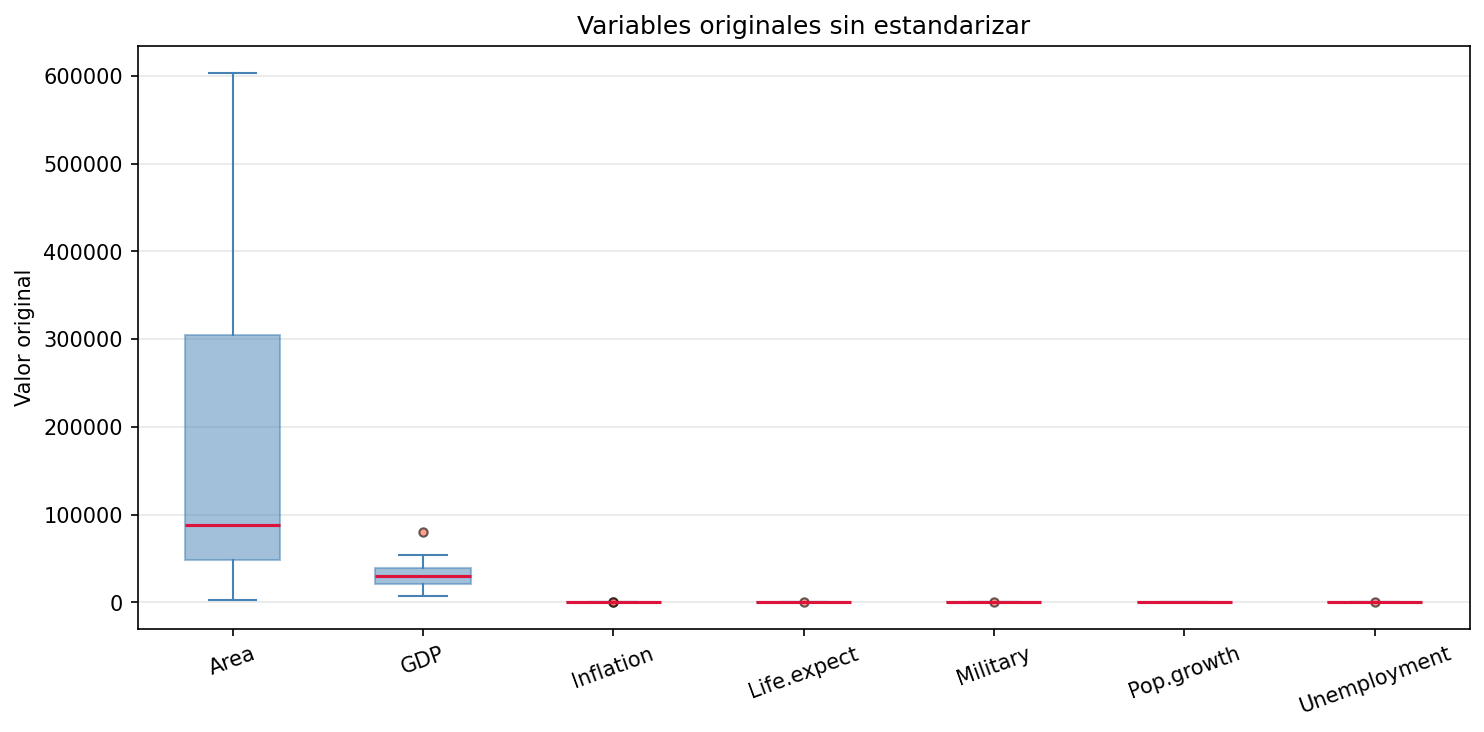
\includegraphics[width=\linewidth]{boxplot_raw}
      \vspace{0.05em}

      \centering
      \small Sin estandarizar
    \end{column}
    \begin{column}{0.5\textwidth}
      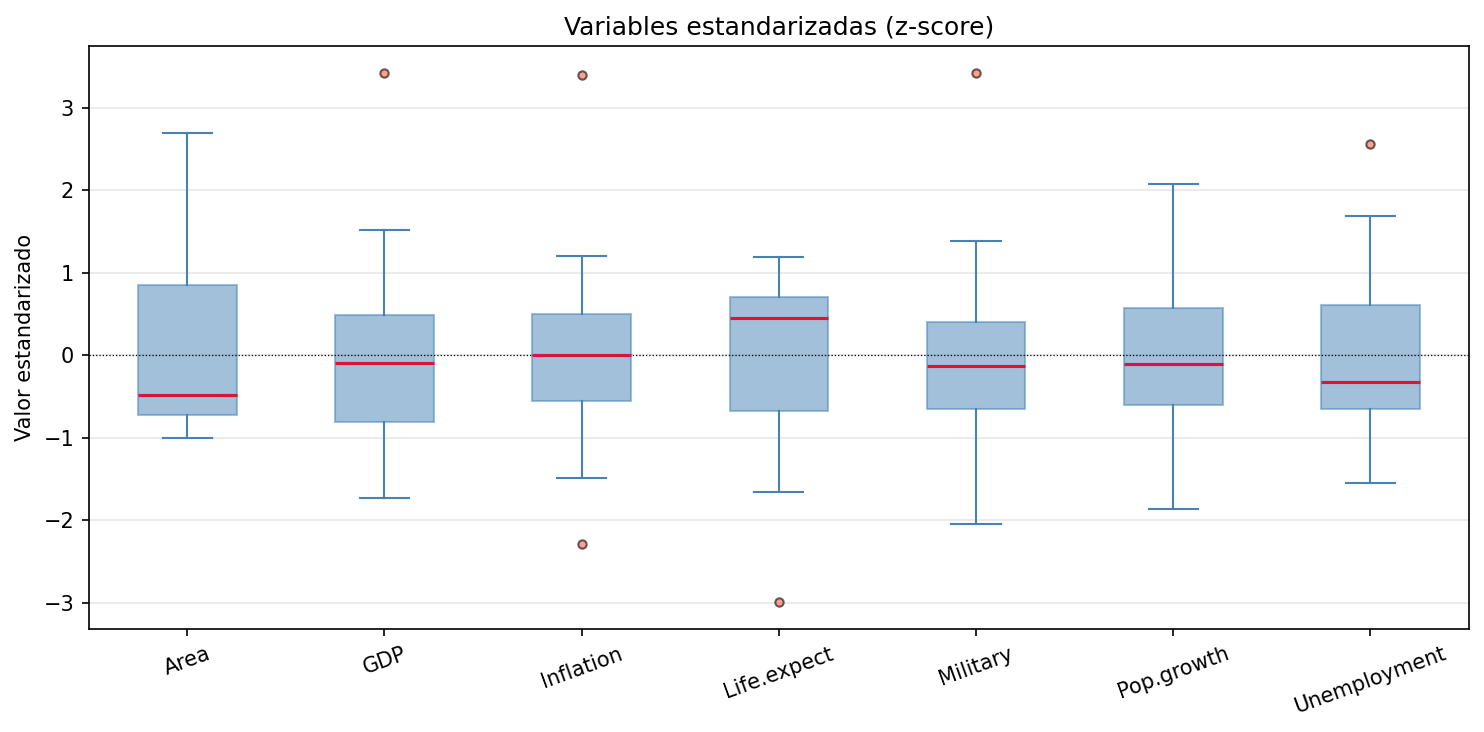
\includegraphics[width=\linewidth]{boxplot_standardized}
      \vspace{0.05em}

      \centering
      \small Con z-score
    \end{column}
  \end{columns}

  \vspace{0.35em}
  \small
  \begin{itemize}
    \item Sin estandarizar, \texttt{Area} y \texttt{GDP} dominan la varianza solo por escala.
    \item Con \textit{z-score}, cada variable queda con media 0 y varianza 1, y todas pasan a ser comparables.
    \item Por eso aplicamos PCA sobre datos estandarizados, equivalente a trabajar sobre la matriz de correlacion.
  \end{itemize}
\end{frame}

\begin{frame}{2. Estructura del dataset: hay relaciones para resumir}
  \begin{columns}[T]
    \begin{column}{0.58\textwidth}
      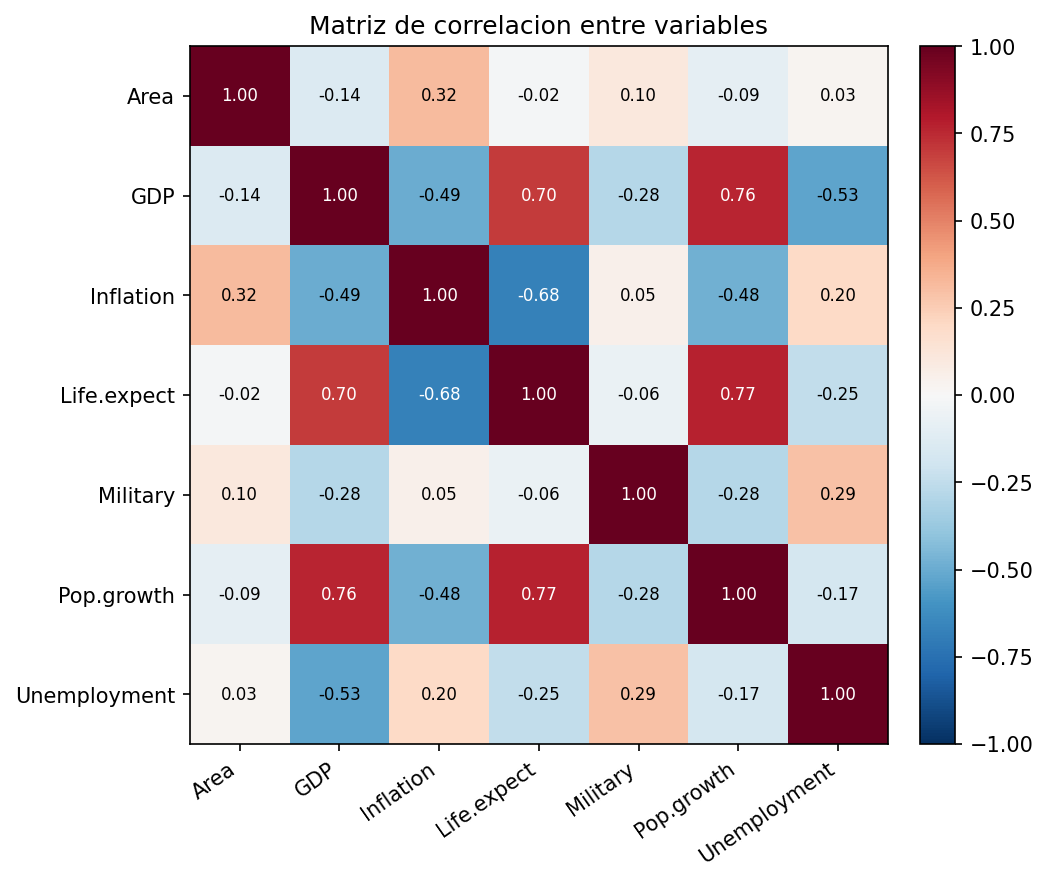
\includegraphics[width=\linewidth]{correlation_heatmap}
    \end{column}
    \begin{column}{0.42\textwidth}
      \small
      \textbf{Idea clave:} hay variables que se mueven juntas.
      \vspace{0.5em}

      \begin{itemize}
        \item \texttt{GDP} y \texttt{Pop.growth}: $r=+0.76$.
        \item \texttt{Life.expect} y \texttt{Pop.growth}: $r=+0.77$.
        \item \texttt{GDP} y \texttt{Life.expect}: $r=+0.70$.
        \item \texttt{Inflation} y \texttt{Life.expect}: $r=-0.68$.
      \end{itemize}

      \vspace{0.4em}
      Entonces tiene sentido buscar nuevas direcciones que concentren la informacion redundante en pocas componentes.
    \end{column}
  \end{columns}
\end{frame}

\begin{frame}{3. Cargas de PC1 y PC2}
  \centering
  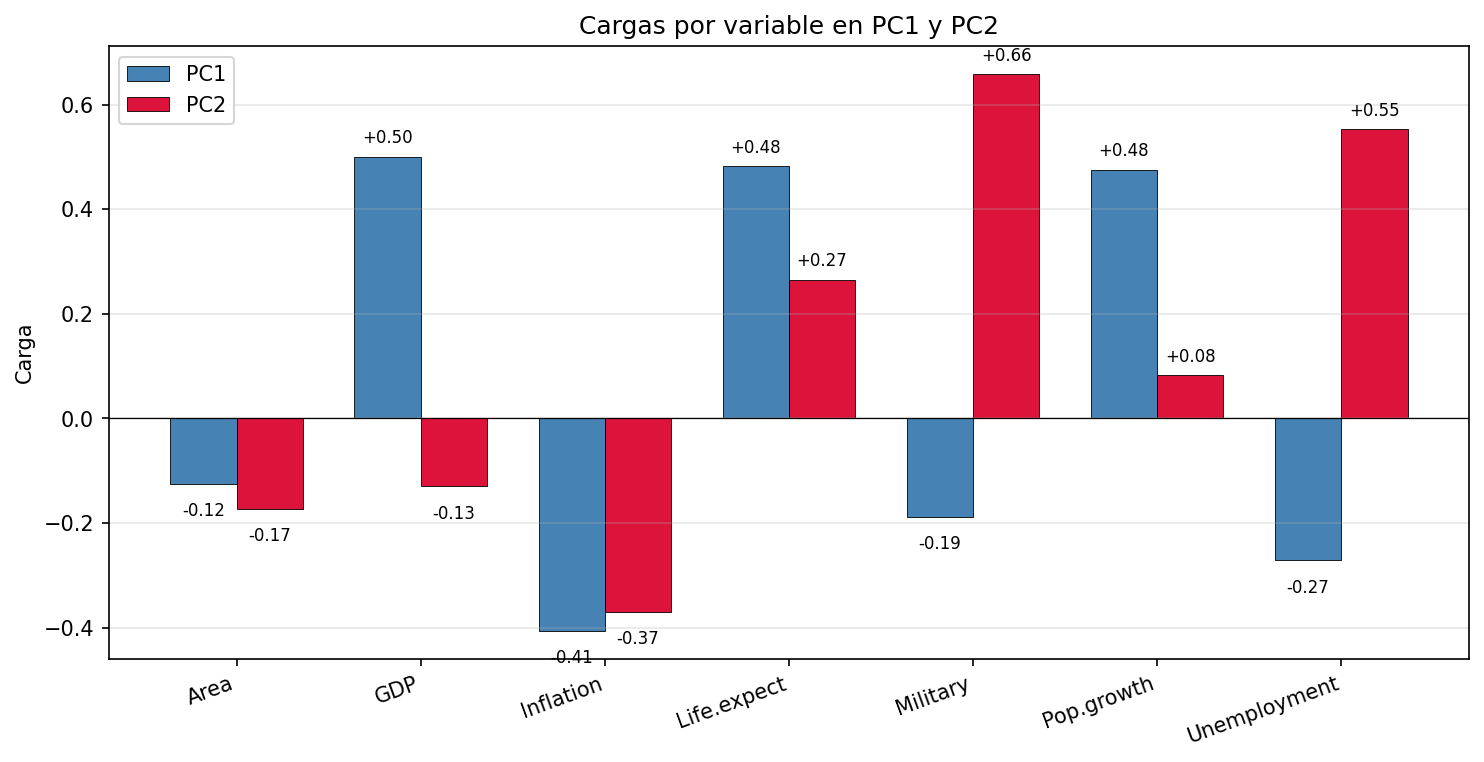
\includegraphics[width=0.82\linewidth,height=0.54\textheight,keepaspectratio]{pc1_pc2_loadings_bars}

  \vspace{0.15em}
  \footnotesize
  \textbf{PC1} favorece \texttt{GDP}, \texttt{Life.expect} y \texttt{Pop.growth}.\\[0.2em]
  \textbf{PC2} pesan fuerte \texttt{Military} y \texttt{Unemployment}.
\end{frame}

\begin{frame}{4. Biplot PC1 vs PC2}
  \centering
  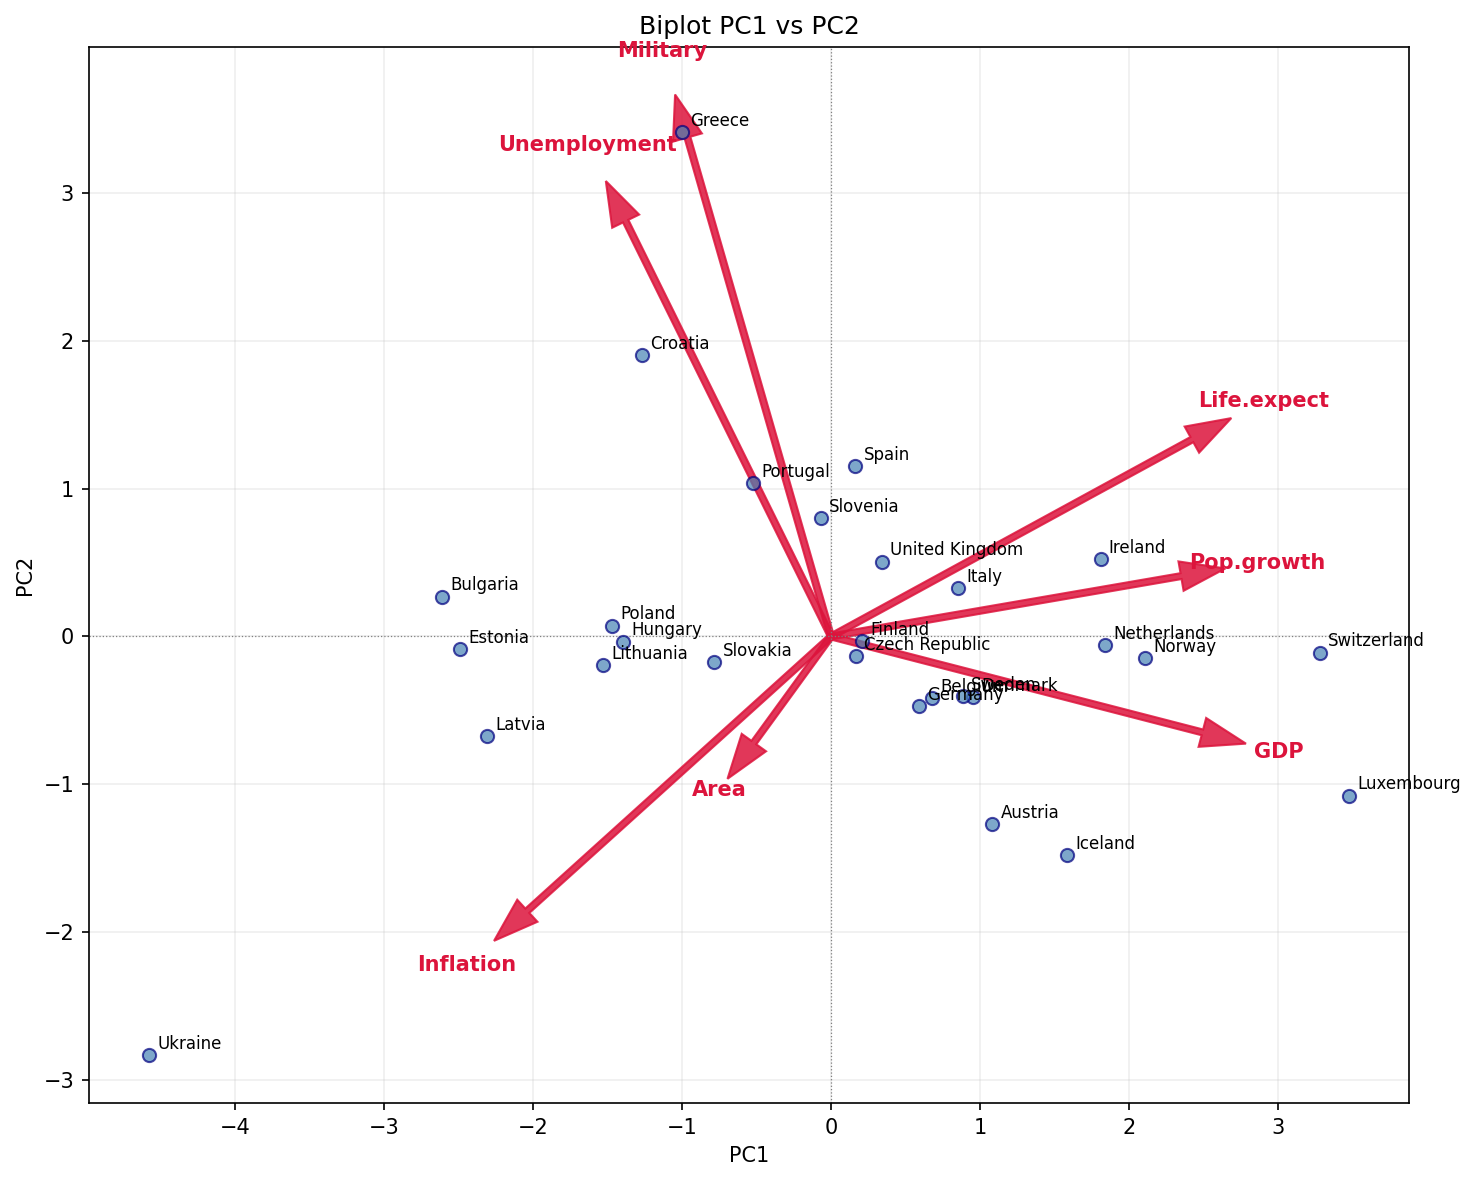
\includegraphics[width=0.92\linewidth,height=0.72\textheight,keepaspectratio]{biplot_pc1_pc2}

  \vspace{0.1em}
  \footnotesize
  Las flechas indican la direccion de cada variable; paises cercanos entre si tienen perfiles similares.
\end{frame}

\end{document}
